\chapter{Projektafgrænsninger}
Dette kapitel beskriver projektets afgrænsninger og hvilke arbejdsopgaver der blevet frasorteres i udviklingsfasen. Afgrænsninger kan både være helt undladt i projektet, eller bestemte faktorer der har begrænset udvikling af vise dele i systemet. 

\section{Sikkerhedskontrol} \label{title:sikkerhedskontrol}
Fra projekts start i forprojektet lå der et ønske fra kundens side omkring en sikkerhedskontrol ved konditioneringsbehandlingen. Fra kundens side bestod ønsket i at kontrollere kredsløbet på patienten, der modtog konditioneringsbehandling. Ønsket lød på at bruge et pulsoximeter som sikkerhedskontrol. Det færdige produkt skulle ved hjælp af et pulsoximeter tjekket patients saturation og puls og ud fra threshold værdier vurdere om patienten kunne tåle behandlingen. De tænkte cases, hvor sikkerhedskontrollen skulle afbryde behandlingen, var ved patienter med dårligt kredsløb, som under behandlingen udvikler koldbrand i den afklemte ekstremitet. Problematikken ved at bruge et pulsoximeter som sikkerhedskontrol ligger i teknikken bag pulsoximeteri. 

Pulsoximeteri måler variationer i det pulserende blod ved at detektere ændringerne i absorption af lys fra to eller flere lyskilder med forskellige bølgelængder. Når væv belyses kan absorptionsgrundlaget opdeles i fire dele (Se figur \ref{fig:opticTissue})
\begin{figure}[H]
	\centering
	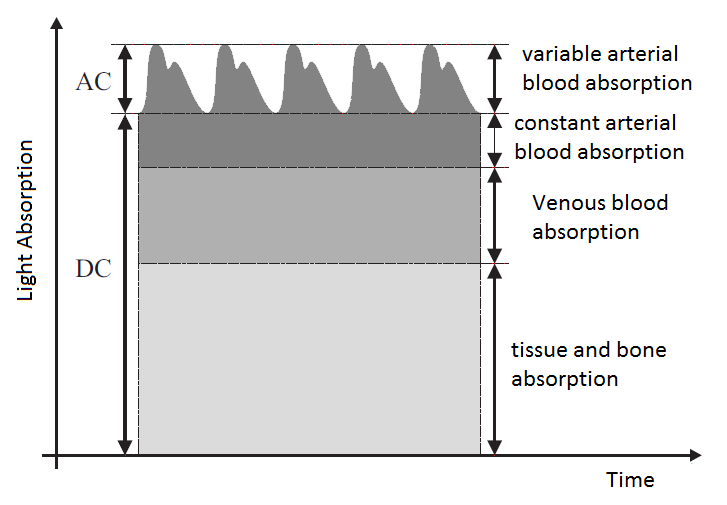
\includegraphics[width = 0.7\textwidth]{billeder/opticTissue.png}
	\caption{Oversigt over absorption af lys i væv}\label{fig:opticTissue}
\end{figure}

I pulsoximeteri filtreres alt DC væk, dvs absorption fra venøst blod, den konstante mængde af arterielt blod og alt andet væv. Det tilbageværende signal, er det pulserende arterielle blod. For at måle saturationen udregnes forskellen på absorption ved \textit{pulstop} og \textit{pulsbund}. Disse absorptioner kan ved hjælp af den molære extinction koefficient for hhv. oxyhæmoglobin og deoxyhæmoglobin og afstanden mellem lyskilde og modtager omregnes til relative koncentrations ændring i hhv. oxyhæmoglobin og deoxyhæmoglobin. Disse relative koncentrations ændringer kan så omsættes til saturation via formlen \ref{eq:satequation}
\begin{equation}
	SaO_2 = \frac{\Delta[HbO_2]}{\Delta[HbO_2]+\Delta[HHb]}
	\label{eq:satequation}
\end{equation}

Efter som at pulseoximetri kun giver indblik i iltmætningen af det pulserende arterielle blod, indeholder den målte iltmætning ikke information angående det lokale væv, men kun information angående respirationen. Pulsoximeteri er derfor en indikator for respirationen og for hvor godt patientens respiratoriske kredsløb forsyner blodet. Appopleksi patienter har som udgangspunkt ikke dårlig respiration, og saturationen af blodet vil derfor ligge over 90\%. Sikkerhedskontrollen skulle kontrollere om iltreserven i armen var nået op på et tilstrækkeligt niveau efter hver afklemning, men eftersom at saturationen ikke er et udtryk for vævet/statisk-blod (iltreserven i armen) kan pulseoximetri ikke måle iltreserven.
Det er heller ikke muligt, at måle AC værdier for det arterielle blod under en afklemning, fordi det pulserende signal er ikke tilstedeværende på grund af okklusionen. Derfor kan selv en person med dårlig kredsløb få målt normal puls og saturation, og stadig tage skade af konditioneringsbehandlingen. 

Denne problemstilling blev opdaget forholdsvis hurtigt i projektforløbet og kunden blev orienteret omkring problemstillingen. Det blev derfor bestemt at projektet skulle afgrænses i forbindelse med sikkerhedskontrollen. Der er gjort plads i udviklingsdokumentation til at implementering af en anden form for sikkerhedskontrol. For at få underbygget påstanden omkring pulsoximeteri og sikkerhedskontrol, har projektgruppen blandt andet været i kontakt med Troels Johansen fra lungemedicinsk afsnit på AUH (Se afsnit \ref{title:samarbejdspartnere} omkring samarbejdspartnere og mødereferater \fixme{Reference til mødereferat med Troels Johansen}). Troels kunne kun bekræfte påstanden omkring at pulsoximeteri som være ugyldig til sikkerhedskontrol, og så i stedet muligheder i NIRS(Se afsnit \ref{title:nirs} i perspektivering) eller at bruge pulsoximeteri som kontrol af om afklemningen var tilstrækkeligt. 

\section{MR kompatibilitet}
I forbindelse med forprojektet var et ønskescenarie fra kunden side at apparatet der skulle udviklings til at udfører konditionering skulle kunne gå i en MR-scanner. Dette var et ønske fordi perkonditionering, hvis det køres i fx 4 cyklusser af 5 minutter, vil tage længere tid at gennemfører, end den tid det tager at kører til hospitalet. Proceduren for patient der mistænkes for have apopleksi er at få dem i MR scanneren så hurtigt så muligt, og derfor kan man i nogle tilfælde være nød til at afbryde konditioneringsbehandlingen og der kan stilles spørgsmålstegn ved den gavnlige effekt. Det blev meget hurtigt bestemt af projektet måtte afgrænse sig fra at lave apparatet MR kompatibel, da dette ville stille alt for høje krav til produktets komponenter og dens håndtering af de ekstremt kraftige elektromagnetiske felter.

\section{Signal behandling}

\section{Seagull samarbejde}
I begyndelse af projektet blev der igennem kunden etableret et sammen arbejdet med en dansk virksomhed, som skulle fungere som talerør til en kinesisk blodtryksapparat producent (Se afsnit \ref{title:samarbejdspartnere} omkring samarbejdspartnere). Tanken bag samarbejdet var at den kinesiske virksomhed skulle kunne bestå med komponenter og teknisks sparringen. Grunden til at den danske virksomhed var med som mellemmand var et ønske fra deres side, da den kinesiske virksomhed var deres kontakt. Et andet argument for at det skulle være sammen arbejde med virksomheder var et ønskede fra kunden side omkring produktet skulle lige sig tæt opad Seagulls apparatet. 

Men efter flere forgæves forsøg for at kommunikere og få information ud af den kinesisk virksomhed blevet det opgivet at produktet skulle ligge sig op af deres apparater. Det forgæves samarbejde betød også at alt arbejdet med \textit{konditioneringsapparatet}, og især udviklingen af en blodtryksalgoritme måtte foretages på egen hånd af projektgruppen selv og uden nogen form for sparring. 

\section{Prototypen}